\documentclass[a4paper,fleqn]{cas-sc}
\usepackage[authoryear]{natbib}
\usepackage{lineno}
\usepackage{booktabs}
\usepackage{url}
\linenumbers

\begin{document}
\let\WriteBookmarks\relax
\def\floatpagepagefraction{1}
\def\textpagefraction{.001}

\shorttitle{Unidade amostral em compósitos do ENSO}
\shortauthors{Y.A.S. Oliveira et al.}

\title[mode = title]{Unidade amostral e significância em compósitos do ENSO: fotossíntese líquida MODIS na Mata Atlântica, no Cerrado e na Caatinga (Bahia, Brasil), 2001--2025}

\author[1]{Ygor Augusto dos Santos Oliveira}[orcid=0009-0001-5821-658X]
\cormark[1]
\ead{ygornayty2@gmail.com}
\credit{Conceituação, Metodologia, Software, Análise formal, Curadoria de dados, Redação -- rascunho original}

\author[1]{Nayanne Silva Benfica}
\credit{Conceituação, Metodologia, Curadoria de dados, Redação -- revisão e edição, Supervisão}

\author[1]{Fabr\'icio Berton Zanchi}[orcid=0000-0002-8074-2893]
\credit{Conceituação, Metodologia, Redação -- revisão e edição, Supervisão}

\affiliation[1]{organization={Programa de Pós-graduação em Ciências e Tecnologias Ambientais, Universidade Federal do Sul da Bahia / Instituto Federal de Educação, Ciência e Tecnologia da Bahia},
  city={Porto Seguro},
  postcode={45810-000},
  state={Bahia},
  country={Brasil}}

\cortext[1]{Autor correspondente}

\begin{abstract}
A associação entre o El Niño--Oscilação Sul (ENSO) e a produtividade da vegetação costuma ser avaliada compondo anomalias mensais por fase e testando-as com procedimentos que tratam cada mês como uma observação independente. Meses de um mesmo episódio, porém, são fortemente autocorrelacionados, e a unidade efetiva de amostragem é o episódio. Este trabalho quantificou a resposta da fotossíntese líquida (PSN, MOD17A2HGF) às fases do ENSO em três biomas da Bahia, Nordeste do Brasil, e avaliou quanto da resposta aparente depende da unidade amostral adotada. Foram usados 297 períodos mensais entre 2001 e 2025, com evapotranspiração, precipitação, temperatura da superfície e um índice de disponibilidade hídrica como covariáveis. As fases oficiais da NOAA correspondem a 76 meses de El Niño distribuídos em 8 episódios, 72 meses de La Niña em 9 sequências e 149 meses neutros. Para a mesma estatística --- a diferença entre a anomalia percentual média da fase e a dos meses neutros --- calcularam-se intervalos de confiança por bootstrap i.i.d.\ sobre meses e por bootstrap em blocos, sorteando episódios inteiros. Sob o esquema convencional, 10 de 30 testes foram significativos; sob o esquema por episódio, 3. Os intervalos alargaram-se 1,67 vez em mediana, chegando a 2,53. Sobreviveram a redução da PSN da Mata Atlântica em El Niño ($-5{,}4$~p.p.; IC95\% $-9{,}2$ a $-0{,}05$), o aquecimento da superfície nesse bioma e fase ($+3{,}1$~p.p.; IC95\% $+0{,}9$ a $+5{,}3$) e o aumento da PSN da Caatinga em La Niña ($+10{,}4$~p.p.; IC95\% $+0{,}4$ a $+16{,}9$). O efeito mais forte do esquema convencional, o aumento de 11,7~p.p.\ da PSN do Cerrado em La Niña ($p = 0{,}003$), deixou de ser significativo ($p = 0{,}081$). Nenhum bioma apresentou tendência interanual significativa entre 2001 e 2024. Os resultados indicam que compósitos do ENSO construídos sobre meses superestimam a significância em séries de sensoriamento remoto e que, em 24 anos de registro, a Bahia dispõe de poucos episódios para sustentar afirmações fortes sobre o efeito do ENSO na produtividade.
\end{abstract}

\begin{keywords}
El Niño--Oscilação Sul \sep fotossíntese líquida \sep MODIS \sep bootstrap em blocos \sep autocorrelação temporal \sep Caatinga
\end{keywords}

\maketitle

\section{Introdução}

O El Niño--Oscilação Sul (ENSO) é o principal modo de variabilidade interanual do sistema climático e organiza boa parte das anomalias de precipitação e de temperatura da América do Sul \citep{ropelewski1987, trenberth1997, grimm2003, grimm2009}. No Nordeste do Brasil, episódios quentes costumam ser associados a redução das chuvas e episódios frios a chuvas acima da média, com intensidade que varia conforme a estação e a posição geográfica \citep{kayano2007, marengo2018}. Como a produtividade da vegetação tropical responde à disponibilidade de água e à demanda evaporativa, é razoável esperar que essa variabilidade climática se propague para os fluxos de carbono \citep{zhao2010, nemani2003}.

Os produtos MODIS tornaram viável acompanhar essa propagação de forma contínua e comparável entre regiões \citep{running2004, running2021gpp}. O procedimento mais comum consiste em remover o ciclo anual da série, classificar cada mês segundo a fase oficial do ENSO e comparar as anomalias das fases quente e fria com as dos meses neutros, usando testes de posição como o de Mann-Whitney ou o de Kruskal-Wallis. O procedimento é simples, transparente e amplamente empregado.

Ele contém, porém, uma premissa que raramente é verificada. Esses testes supõem que as observações de cada grupo sejam independentes. Os meses classificados como El Niño não são observações independentes: pertencem a um pequeno número de episódios, cada um com vários meses consecutivos, e tanto o forçante oceânico quanto a resposta da vegetação são fortemente autocorrelacionados dentro de um mesmo episódio. A unidade efetiva de amostragem é o episódio, não o mês. Quando essa distinção é ignorada, o tamanho amostral é inflado por um fator próximo à duração média dos episódios, os intervalos de confiança estreitam e valores de $p$ pequenos são obtidos com facilidade. O problema é conhecido na literatura estatística e climatológica \citep{kunsch1989, politis1994} e tem solução padrão --- reamostrar blocos em vez de observações isoladas ---, mas seu efeito prático sobre compósitos de produtividade derivados de sensoriamento remoto raramente é quantificado.

O estado da Bahia oferece um contexto favorável para esse exame. Em cerca de 565 mil km$^2$ reúne três biomas dispostos ao longo de um gradiente hidroclimático contínuo, da Mata Atlântica úmida no litoral à Caatinga semiárida no interior, com o Cerrado na posição intermediária \citep{ibge2019, alvares2013}. Os três compartilham o mesmo forçante remoto e o mesmo protocolo de extração de dados, o que permite comparar respostas sem confundir bioma com metodologia. A produtividade desses biomas e sua relação com fatores climáticos e antrópicos já foi descrita para a região \citep{benfica2022, benfica2023}, e um modelo de regressão polinomial regularizada da PSN mensal foi desenvolvido e validado para os mesmos três biomas e o mesmo período \citep{oliveira2026}.

Este trabalho tem dois objetivos. O primeiro é quantificar a resposta da fotossíntese líquida às fases do ENSO nos três biomas, incluindo a defasagem da resposta e a fração dela que o modelo climático reproduz por meio dos preditores. O segundo, e principal, é medir quanto dessa resposta depende da unidade amostral adotada, comparando, para a mesma estatística, o esquema convencional baseado em meses e um esquema em que a unidade é o episódio.

\section{Material e métodos}

\subsection{Área de estudo}

A área compreende as porções baianas da Mata Atlântica, do Cerrado e da Caatinga, delimitadas pelo mapa de biomas do IBGE na escala 1:250.000 recortado pelo limite estadual \citep{ibge2019}. O gradiente hidroclimático vai de Af/Am no litoral a BSh no interior semiárido, com precipitação média anual de cerca de 1.400~mm na Mata Atlântica, 1.000~mm no Cerrado e 600~mm na Caatinga \citep{alvares2013}. A descrição detalhada dos biomas e do protocolo de extração consta de \citet{oliveira2026}.

\subsection{Dados}

A série mensal cobre janeiro de 2001 a setembro de 2025, com 297 períodos por bioma. Cada período é uma janela fixa de quatro compósitos consecutivos de oito dias, atribuída ao mês civil que contém a maior parte de seus dias. A fotossíntese líquida (PSN) provém do MOD17A2HGF C6.1 \citep{running2021gpp}; a evapotranspiração real (EV) e a potencial, do MOD16A2GF C6.1 \citep{running2021et}; a temperatura diurna da superfície (TST), do MOD11A2 C6.1 \citep{wan2021}; e a precipitação (PRE), do GPM IMERG Final Run V07 \citep{huffman2023}. O índice de disponibilidade hídrica (WAI) é a razão entre evapotranspiração real e potencial. As médias espaciais foram calculadas sobre os pixels válidos de cada bioma no Google Earth Engine \citep{gorelick2017}.

O Índice Oceânico Niño (ONI) foi obtido da tabela completa do Climate Prediction Center da NOAA \citep{noaacpc2025}. A classificação das fases segue o critério oficial: El Niño quando o ONI permanece em $+0{,}5$~$^{\circ}$C ou acima por cinco trimestres consecutivos sobrepostos, La Niña quando permanece em $-0{,}5$~$^{\circ}$C ou abaixo pelo mesmo intervalo, e Neutro nos demais casos.

\subsection{Anomalias}

Para cada variável e bioma, a climatologia é a média do mês civil correspondente ao longo de toda a série, e a anomalia é expressa em porcentagem dessa climatologia. A remoção do ciclo anual é necessária porque as fases do ENSO não se distribuem uniformemente pelo calendário: os episódios ativos concentram-se no verão austral, de modo que uma comparação sobre valores brutos confundiria fase e estação. A assimetria é acentuada: os meses de El Niño representam de 10,5\% a 11,8\% da amostra entre novembro e fevereiro, mas apenas de 3,9\% a 5,3\% entre maio e julho, ao passo que os meses neutros seguem a distribuição inversa (4,0\% e 12,8\%, respectivamente).

\subsection{Análise convencional}

A anomalia de cada fase ativa foi comparada à dos meses neutros pelo teste de Mann-Whitney, e as três fases pelo teste de Kruskal-Wallis, com o tamanho de efeito $\varepsilon^2$. A homogeneidade da dispersão foi avaliada pelo teste de Fligner-Killeen e a frequência de extremos por um teste qui-quadrado sobre a proporção de meses abaixo do percentil 10 e acima do percentil 90 da própria série de anomalias. Os valores de $p$ desses quatro conjuntos de testes foram corrigidos para comparações múltiplas pelo procedimento de Benjamini-Hochberg, controlando a taxa de falsas descobertas em 5\% \citep{benjamini1995}. Este é o procedimento que se toma aqui como referência do uso corrente, e todos os seus resultados são reportados.

\subsection{Unidade amostral}

A estatística de interesse é a diferença entre a anomalia percentual média de uma fase ativa e a dos meses neutros. Para essa mesma estatística foram calculados dois intervalos de confiança de 95\%, ambos por percentis de 10.000 reamostragens, com a mesma semente:

\begin{enumerate}
  \item \emph{mês como unidade}: bootstrap i.i.d., sorteando meses com reposição dentro de cada grupo, que é o esquema implícito nos testes da seção anterior;
  \item \emph{episódio como unidade}: bootstrap em blocos, sorteando com reposição sequências contíguas inteiras de meses da mesma fase \citep{kunsch1989, politis1994}, o que preserva a dependência interna de cada episódio.
\end{enumerate}

Os blocos foram definidos como corridas contíguas de meses na mesma fase oficial, sem imposição de comprimento: cada bloco é um episódio do ENSO tal como a NOAA o delimita. O valor de $p$ do bootstrap é bilateral, obtido da proporção da distribuição reamostrada que cruza zero. Os dois esquemas foram aplicados à PSN e aos quatro preditores nos três biomas, totalizando 30 testes.

\subsection{Defasagem}

A resposta defasada foi avaliada pela correlação de Spearman entre o ONI do mês $t$ e a anomalia de PSN do mês $t+L$, para $L$ de 0 a 12 meses. Essas correlações usam o mês como unidade e são apresentadas como parte da caracterização convencional, com a ressalva que decorre das seções anteriores.

\subsection{Mediação pelo modelo climático}

Para estimar que fração da resposta da PSN é explicada pelas variáveis climáticas medidas, usou-se o modelo de regressão polinomial de grau 2 com regularização de Ridge ajustado para os mesmos biomas e período \citep{oliveira2026, hoerl1970}. Para cada bioma e fase, a anomalia média observada em cada preditor foi imposta ao modelo, isoladamente e em conjunto, e a resposta predita da PSN foi comparada à observada.

\subsection{Variabilidade interanual}

A PSN anual é a soma dos períodos de cada ano. A tendência foi estimada pelo declive de Sen \citep{sen1968} e testada por Mann-Kendall \citep{mann1945}, com intervalo de confiança por bootstrap. O ano de 2025, com nove períodos disponíveis, foi excluído do cálculo de tendência e tratado separadamente.

Todas as análises foram feitas em Python 3.11 com \texttt{numpy}, \texttt{pandas}, \texttt{scipy} e \texttt{scikit-learn}.

\section{Resultados}

\subsection{Composição das fases}

Dos 297 períodos da série, 76 foram classificados como El Niño, 72 como La Niña e 149 como neutros. Esses meses distribuem-se, porém, em poucas sequências contíguas: 8 episódios de El Niño, 9 sequências de La Niña --- uma das quais truncada no início da série, em janeiro e fevereiro de 2001 --- e 17 intervalos neutros (Tabela~\ref{tab:fases}). A duração das sequências ativas vai de 2 a 20 meses, com mediana de 8 meses. A razão entre o número de meses e o número de episódios, próxima de 9 para o El Niño e de 8 para a La Niña, é a ordem de grandeza do fator pelo qual o tamanho amostral é inflado quando o mês é tomado como unidade.

\begin{table}[width=\linewidth,cols=5,pos=h]
\caption{Composição das fases do ENSO na série mensal de 2001 a 2025, segundo o critério oficial da NOAA.}
\label{tab:fases}
\begin{tabular*}{\tblwidth}{@{}lrrrr@{}}
\toprule
Fase & Meses & Sequências & \multicolumn{2}{c}{Duração (meses)} \\
\cmidrule(l){4-5}
 & & & mediana & mín--máx \\
\midrule
El Niño & 76  & 8  & 8,5 & 5--20 \\
Neutro  & 149 & 17 & 7   & 1--30 \\
La Niña & 72  & 9  & 7   & 2--17 \\
\midrule
Total   & 297 & 34 & --- & --- \\
\bottomrule
\end{tabular*}
\end{table}

A Figura~\ref{fig:episodios} mostra a série de anomalias de PSN dos três biomas com os episódios sombreados. A variabilidade mensal é alta em todos os biomas --- amplitude de cerca de $\pm 40\%$ na Mata Atlântica e de $\pm 90\%$ no Cerrado --- e os episódios do ENSO não se destacam visualmente do restante da série, com a exceção do El Niño de 2014--2016, que coincide com as anomalias negativas mais profundas da Mata Atlântica.

\begin{figure}[pos=h]
\centering
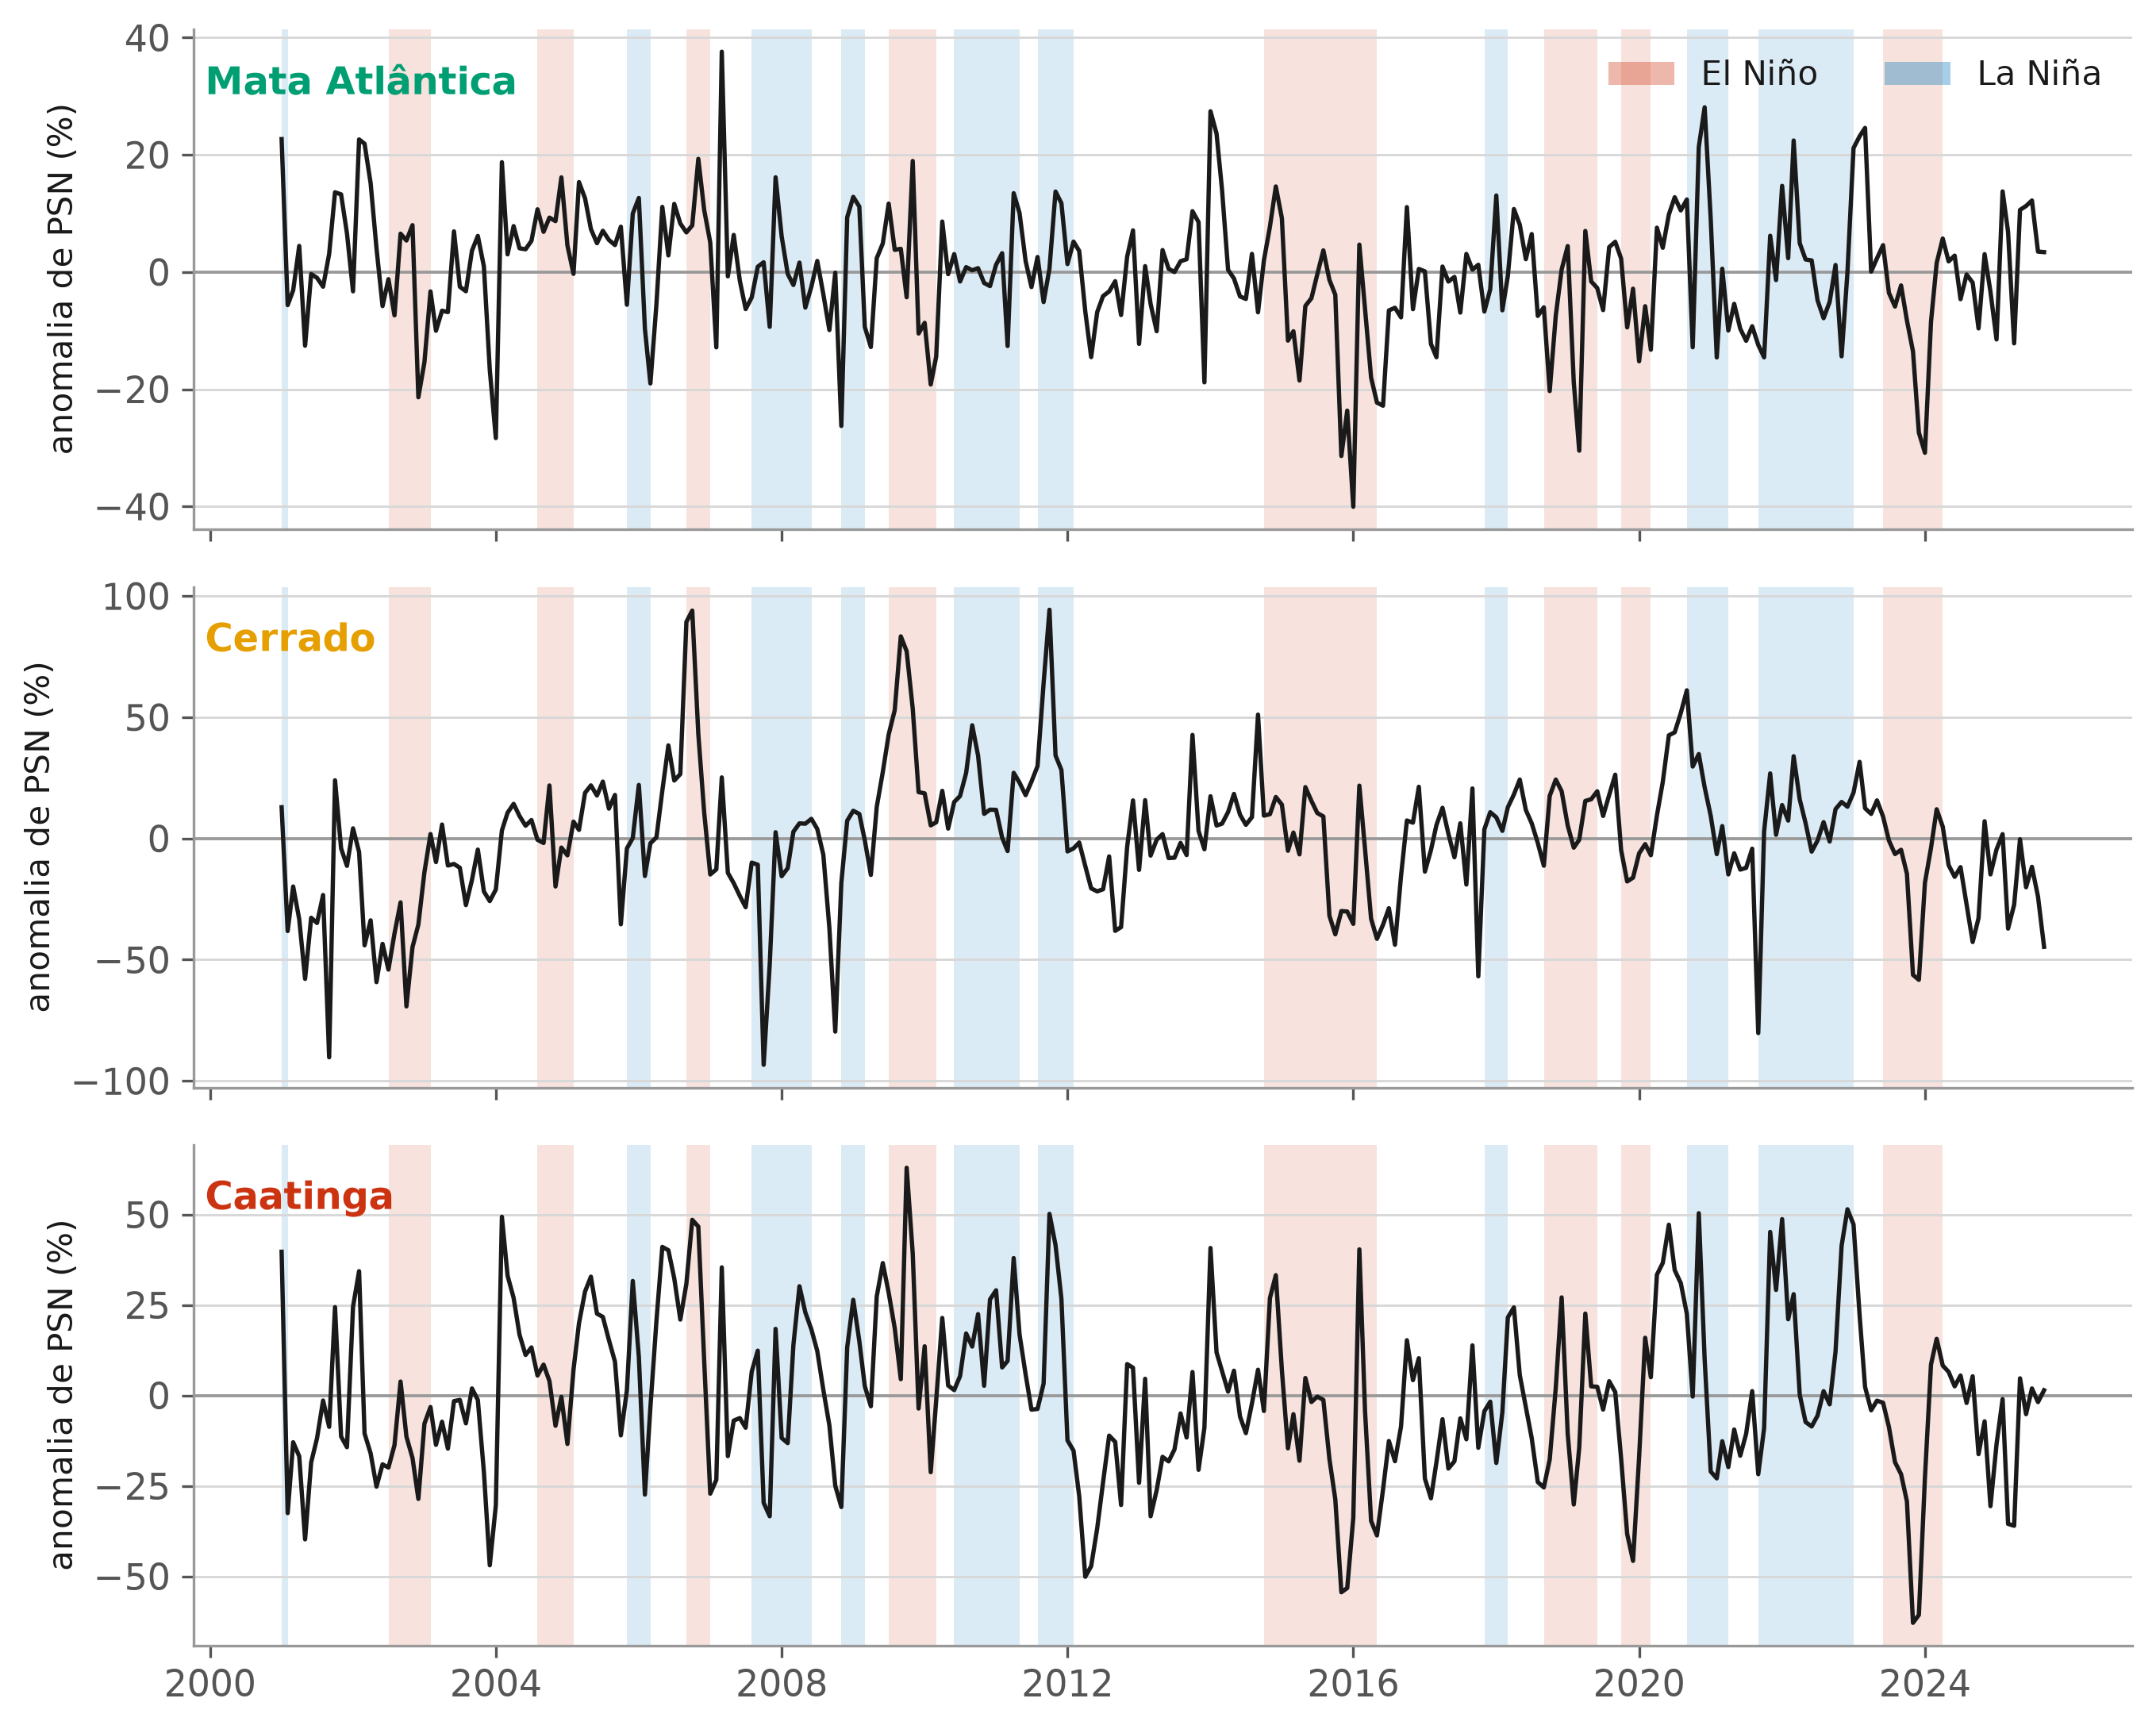
\includegraphics[width=\linewidth]{figs/fig1_episodios.png}
\caption{Anomalia percentual mensal da fotossíntese líquida nos três biomas entre 2001 e 2025, com os episódios de El Niño e de La Niña sombreados. As escalas verticais diferem entre os painéis.}
\label{fig:episodios}
\end{figure}

\subsection{Análise convencional}

Tomando o mês como unidade, a PSN diferiu entre as fases nos três biomas, com um padrão assimétrico (Tabela~\ref{tab:convencional}). Na Mata Atlântica, a anomalia média foi 5,4 pontos percentuais menor em El Niño do que em meses neutros ($p = 0{,}010$), enquanto a La Niña não se distinguiu do neutro ($-0{,}1$ p.p.; $p = 0{,}794$). No Cerrado e na Caatinga ocorreu o inverso: a La Niña elevou a anomalia em 11,7 p.p.\ ($p = 0{,}001$) e 10,4 p.p.\ ($p = 0{,}002$), respectivamente, e o El Niño não produziu diferença detectável. Os três efeitos sobreviveram à correção de Benjamini-Hochberg.

A frequência de extremos acompanhou esse padrão. Na Mata Atlântica, 22,4\% dos meses de El Niño ficaram abaixo do percentil 10 da série, contra 4,7\% dos meses neutros ($p = 0{,}0004$, significativo após correção). As medianas brutas de PSN, porém, são praticamente iguais nas três fases (133,3, 134,3 e 133,8~gC~m$^{-2}$ por período), e o mínimo observado sob El Niño (79,0) fica 15~gC~m$^{-2}$ abaixo do mínimo dos meses neutros (94,4): nesse bioma o El Niño atua sobre a cauda inferior da distribuição, não sobre o seu centro. No Cerrado e na Caatinga, a La Niña deslocou a distribuição inteira para cima: o primeiro quartil do Cerrado sobe de 65,1 para 85,8~gC~m$^{-2}$ e a mediana da Caatinga de 82,4 para 94,6~gC~m$^{-2}$. A proporção de meses acima do percentil 90 é de 12,5\% e 15,3\% em La Niña, contra 7,4\% e 10,1\% nos meses neutros, mas essas diferenças não sobreviveram à correção.

Entre os preditores, o sinal mais forte foi o aquecimento da superfície da Mata Atlântica em El Niño ($+3{,}1$~p.p., ou cerca de 0,9~$^{\circ}$C; $p < 0{,}001$), com 25\% desses meses no decil mais quente da série contra 5\% dos meses neutros. A evapotranspiração e o índice de disponibilidade hídrica aumentaram em La Niña no Cerrado e na Caatinga, com magnitudes entre 10 e 14 p.p. A precipitação não apresentou diferença significativa entre fases em nenhum bioma. As médias brutas sugeririam o contrário: no Cerrado, os meses de La Niña acumulam 123~mm por período e os de El Niño 107~mm, contra 59~mm nos meses neutros, e o contraste se repete na Caatinga (73 e 66 contra 46~mm). Como as duas fases ativas superam a neutra na mesma direção, trata-se do efeito de calendário antecipado na Seção~2.3: no Cerrado, a diferença de 64~mm entre La Niña e meses neutros cai para 8~mm quando o ciclo anual é removido.

\begin{table*}[width=\textwidth,cols=7,pos=t]
\caption{Anomalia percentual média de cada fase ativa em relação aos meses neutros, com o valor de $p$ do teste de Mann-Whitney tomando o mês como unidade. Em negrito, os resultados que sobreviveram à correção de Benjamini-Hochberg (taxa de falsas descobertas de 5\%).}
\label{tab:convencional}
\begin{tabular*}{\tblwidth}{@{}llrrrr@{}}
\toprule
Bioma & Variável & \multicolumn{2}{c}{El Niño} & \multicolumn{2}{c}{La Niña} \\
\cmidrule(lr){3-4}\cmidrule(l){5-6}
 & & $\Delta$ (p.p.) & $p$ & $\Delta$ (p.p.) & $p$ \\
\midrule
Mata Atlântica & PSN & $\mathbf{-5{,}44}$ & \textbf{0,010} & $-0{,}08$ & 0,794 \\
               & EV  & $-1{,}52$ & 0,488 & $+1{,}37$ & 0,359 \\
               & PRE & $-5{,}28$ & 0,181 & $-1{,}27$ & 0,888 \\
               & TST & $\mathbf{+3{,}07}$ & $\mathbf{<0{,}001}$ & $-0{,}50$ & 0,322 \\
               & WAI & $-2{,}49$ & 0,189 & $+2{,}44$ & 0,182 \\
\addlinespace
Cerrado        & PSN & $+5{,}26$ & 0,375 & $\mathbf{+11{,}75}$ & \textbf{0,001} \\
               & EV  & $+7{,}51$ & 0,080 & $\mathbf{+10{,}22}$ & $\mathbf{<0{,}001}$ \\
               & PRE & $+7{,}91$ & 0,875 & $-7{,}73$ & 0,461 \\
               & TST & $+1{,}35$ & 0,217 & $-1{,}11$ & 0,050 \\
               & WAI & $+7{,}70$ & 0,245 & $\mathbf{+13{,}99}$ & $\mathbf{<0{,}001}$ \\
\addlinespace
Caatinga       & PSN & $-3{,}28$ & 0,458 & $\mathbf{+10{,}45}$ & \textbf{0,002} \\
               & EV  & $+0{,}34$ & 0,630 & $\mathbf{+10{,}85}$ & \textbf{0,003} \\
               & PRE & $+2{,}54$ & 0,761 & $+4{,}69$ & 0,837 \\
               & TST & $+1{,}51$ & 0,105 & $\mathbf{-2{,}14}$ & \textbf{0,013} \\
               & WAI & $+0{,}43$ & 0,534 & $\mathbf{+12{,}47}$ & \textbf{0,002} \\
\bottomrule
\end{tabular*}
\end{table*}

\subsection{Efeito da unidade amostral}

Repetindo o cálculo com o episódio como unidade, a maior parte desses efeitos deixa de ser distinguível de zero. Dos 30 testes realizados, 10 tiveram intervalo que exclui o zero com o mês como unidade e 3 com o episódio (Tabela~\ref{tab:unidade}, Figura~\ref{fig:unidade}). Esse conjunto de dez contém os nove efeitos que sobreviveram à correção de Benjamini-Hochberg na Tabela~\ref{tab:convencional}, mais a evapotranspiração do Cerrado em El Niño. A largura mediana do intervalo de confiança passou de 12,9 para 23,1 pontos percentuais, um alargamento de 1,67 vez em mediana, que chegou a 2,53 vezes no Cerrado em El Niño.

\begin{table*}[width=\textwidth,cols=8,pos=t]
\caption{Os dez efeitos cujo intervalo de confiança exclui o zero sob o esquema convencional, recalculados com o episódio como unidade amostral. $\Delta$ é a mesma estatística nos dois esquemas; o que muda é a reamostragem. Em negrito, os três que permanecem significativos.}
\label{tab:unidade}
\begin{tabular*}{\tblwidth}{@{}lllrrrrr@{}}
\toprule
 & & & & \multicolumn{2}{c}{Mês como unidade} & \multicolumn{2}{c}{Episódio como unidade} \\
\cmidrule(lr){5-6}\cmidrule(l){7-8}
Bioma & Var. & Fase & $\Delta$ (p.p.) & IC95\% & $p$ & IC95\% & $p$ \\
\midrule
Mata Atlântica & PSN & El Niño & $-5{,}44$  & $-8{,}7$ a $-2{,}3$ & 0,001 & $\mathbf{-9{,}2}$ \textbf{a} $\mathbf{-0{,}05}$ & \textbf{0,048} \\
Mata Atlântica & TST & El Niño & $+3{,}07$  & $+1{,}7$ a $+4{,}4$ & $<0{,}001$ & $\mathbf{+0{,}9}$ \textbf{a} $\mathbf{+5{,}3}$ & \textbf{0,005} \\
Caatinga       & PSN & La Niña & $+10{,}45$ & $+4{,}4$ a $+16{,}4$ & 0,001 & $\mathbf{+0{,}4}$ \textbf{a} $\mathbf{+16{,}9}$ & \textbf{0,044} \\
\addlinespace
Cerrado        & PSN & La Niña & $+11{,}75$ & $+4{,}3$ a $+18{,}9$ & 0,003 & $-1{,}5$ a $+24{,}3$ & 0,081 \\
Cerrado        & WAI & La Niña & $+13{,}99$ & $+6{,}8$ a $+21{,}1$ & $<0{,}001$ & $-2{,}6$ a $+27{,}9$ & 0,087 \\
Cerrado        & EV  & La Niña & $+10{,}22$ & $+4{,}3$ a $+15{,}8$ & 0,001 & $-3{,}5$ a $+21{,}5$ & 0,135 \\
Cerrado        & EV  & El Niño & $+7{,}51$  & $+0{,}6$ a $+14{,}5$ & 0,031 & $-6{,}8$ a $+23{,}2$ & 0,322 \\
Caatinga       & WAI & La Niña & $+12{,}47$ & $+5{,}2$ a $+19{,}6$ & 0,001 & $-2{,}2$ a $+22{,}0$ & 0,086 \\
Caatinga       & EV  & La Niña & $+10{,}85$ & $+4{,}5$ a $+17{,}2$ & 0,001 & $-2{,}2$ a $+19{,}8$ & 0,103 \\
Caatinga       & TST & La Niña & $-2{,}14$  & $-3{,}7$ a $-0{,}6$ & 0,008 & $-5{,}2$ a $+2{,}1$ & 0,327 \\
\bottomrule
\end{tabular*}
\end{table*}

\begin{figure}[pos=h]
\centering
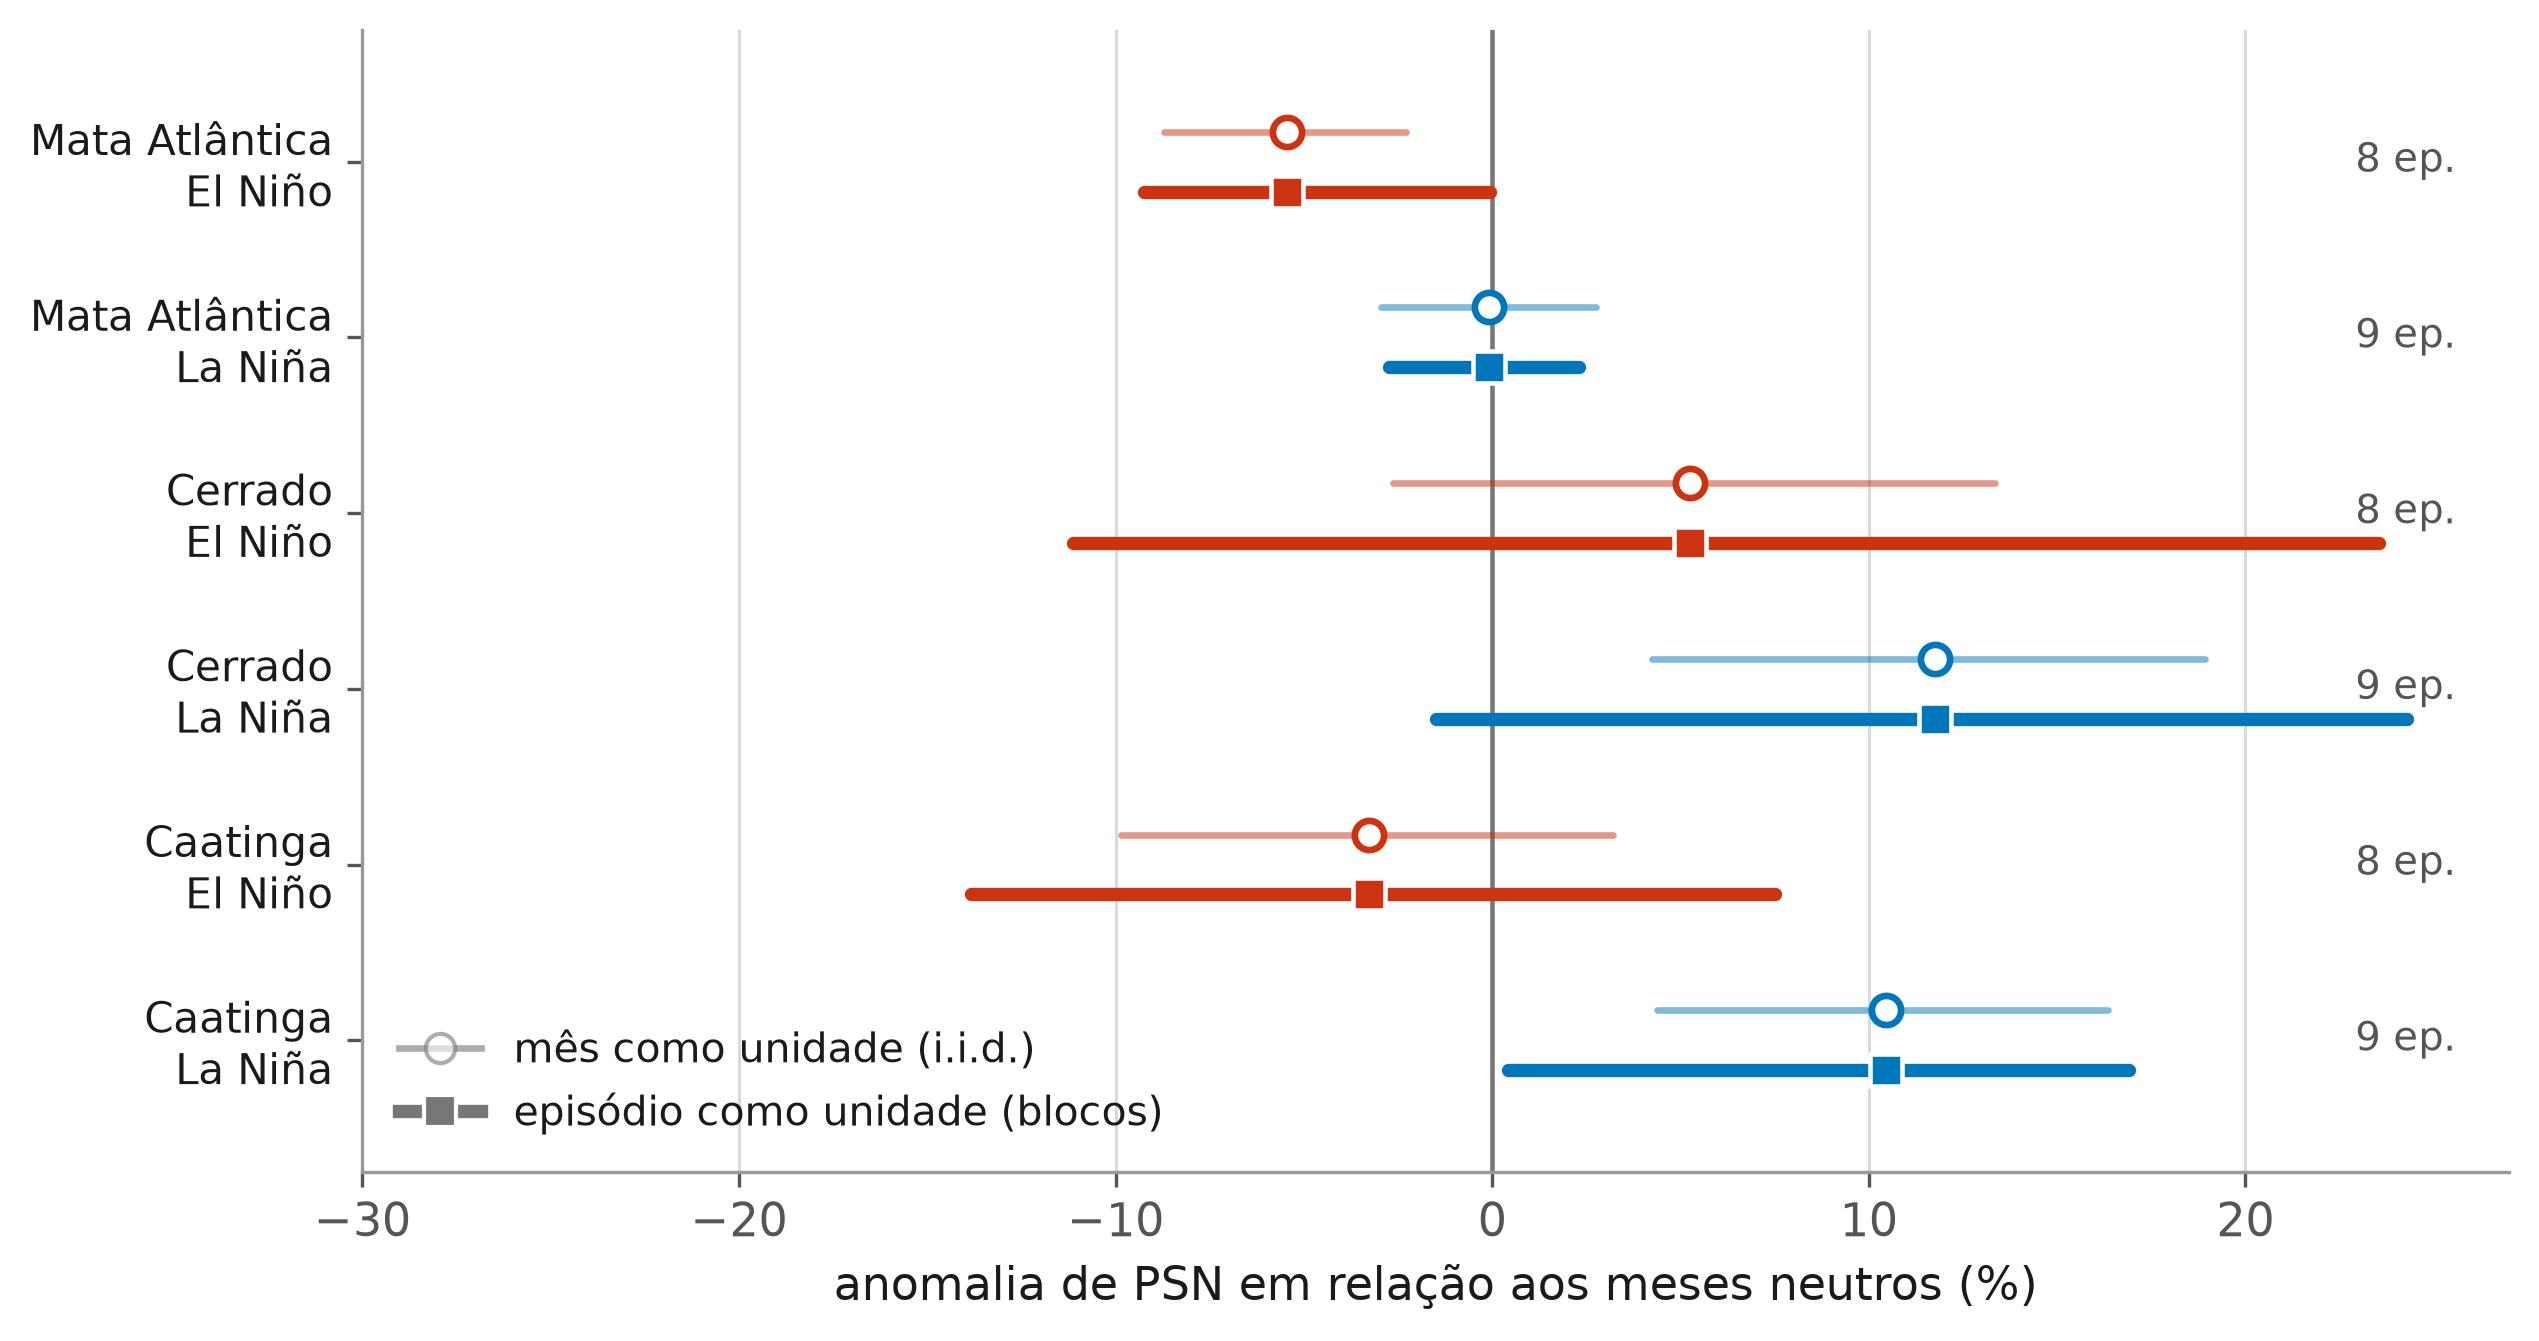
\includegraphics[width=\linewidth]{figs/fig2_unidade.png}
\caption{Anomalia de PSN de cada fase em relação aos meses neutros, com intervalos de confiança de 95\% obtidos por bootstrap sobre meses (linha fina, círculo aberto) e por bootstrap em blocos sobre episódios (linha grossa, quadrado). O número de episódios de cada fase consta à direita.}
\label{fig:unidade}
\end{figure}

Os três efeitos que permaneceram significativos são o aquecimento da superfície da Mata Atlântica em El Niño ($+3{,}07$~p.p.; IC95\% $+0{,}9$ a $+5{,}3$; $p = 0{,}005$), o mais robusto do conjunto, a redução da PSN desse mesmo bioma e fase ($-5{,}44$~p.p.; IC95\% $-9{,}2$ a $-0{,}05$; $p = 0{,}048$) e o aumento da PSN da Caatinga em La Niña ($+10{,}45$~p.p.; IC95\% $+0{,}4$ a $+16{,}9$; $p = 0{,}044$). Os dois últimos são marginais: seus intervalos quase tocam zero.

A mudança mais expressiva ocorreu no Cerrado. O aumento de 11,7~p.p.\ da PSN em La Niña, que sob o esquema convencional tem $p = 0{,}003$ e sobrevive à correção para comparações múltiplas, passa a $p = 0{,}081$ com intervalo de $-1{,}5$ a $+24{,}3$~p.p.\ quando os nove episódios de La Niña são tomados como as nove observações que de fato são. O mesmo ocorre com o índice de disponibilidade hídrica e a evapotranspiração nesse bioma. Na Caatinga, apenas a PSN resiste: evapotranspiração, disponibilidade hídrica e temperatura da superfície, todas significativas com o mês como unidade, deixam de ser.

\subsection{Defasagem}

As correlações entre o ONI e a anomalia de PSN são negativas em todas as defasagens e em todos os biomas, com magnitude entre 0,03 e 0,19 (Figura~\ref{fig:defasagem}). A defasagem de maior correlação difere entre os biomas: a Caatinga responde em fase, com o máximo em $L = 0$ ($\rho = -0{,}19$); a Mata Atlântica, com dois meses de atraso ($\rho = -0{,}16$); e o Cerrado, com dez meses ($\rho = -0{,}16$), permanecendo a correlação praticamente constante entre $L = 1$ e $L = 12$. Mesmo nos máximos, o coeficiente ao quadrado não ultrapassa 3,6\% da variância das anomalias, e os valores de $p$ assinalados na figura compartilham a premissa de independência discutida acima.

\begin{figure}[pos=h]
\centering
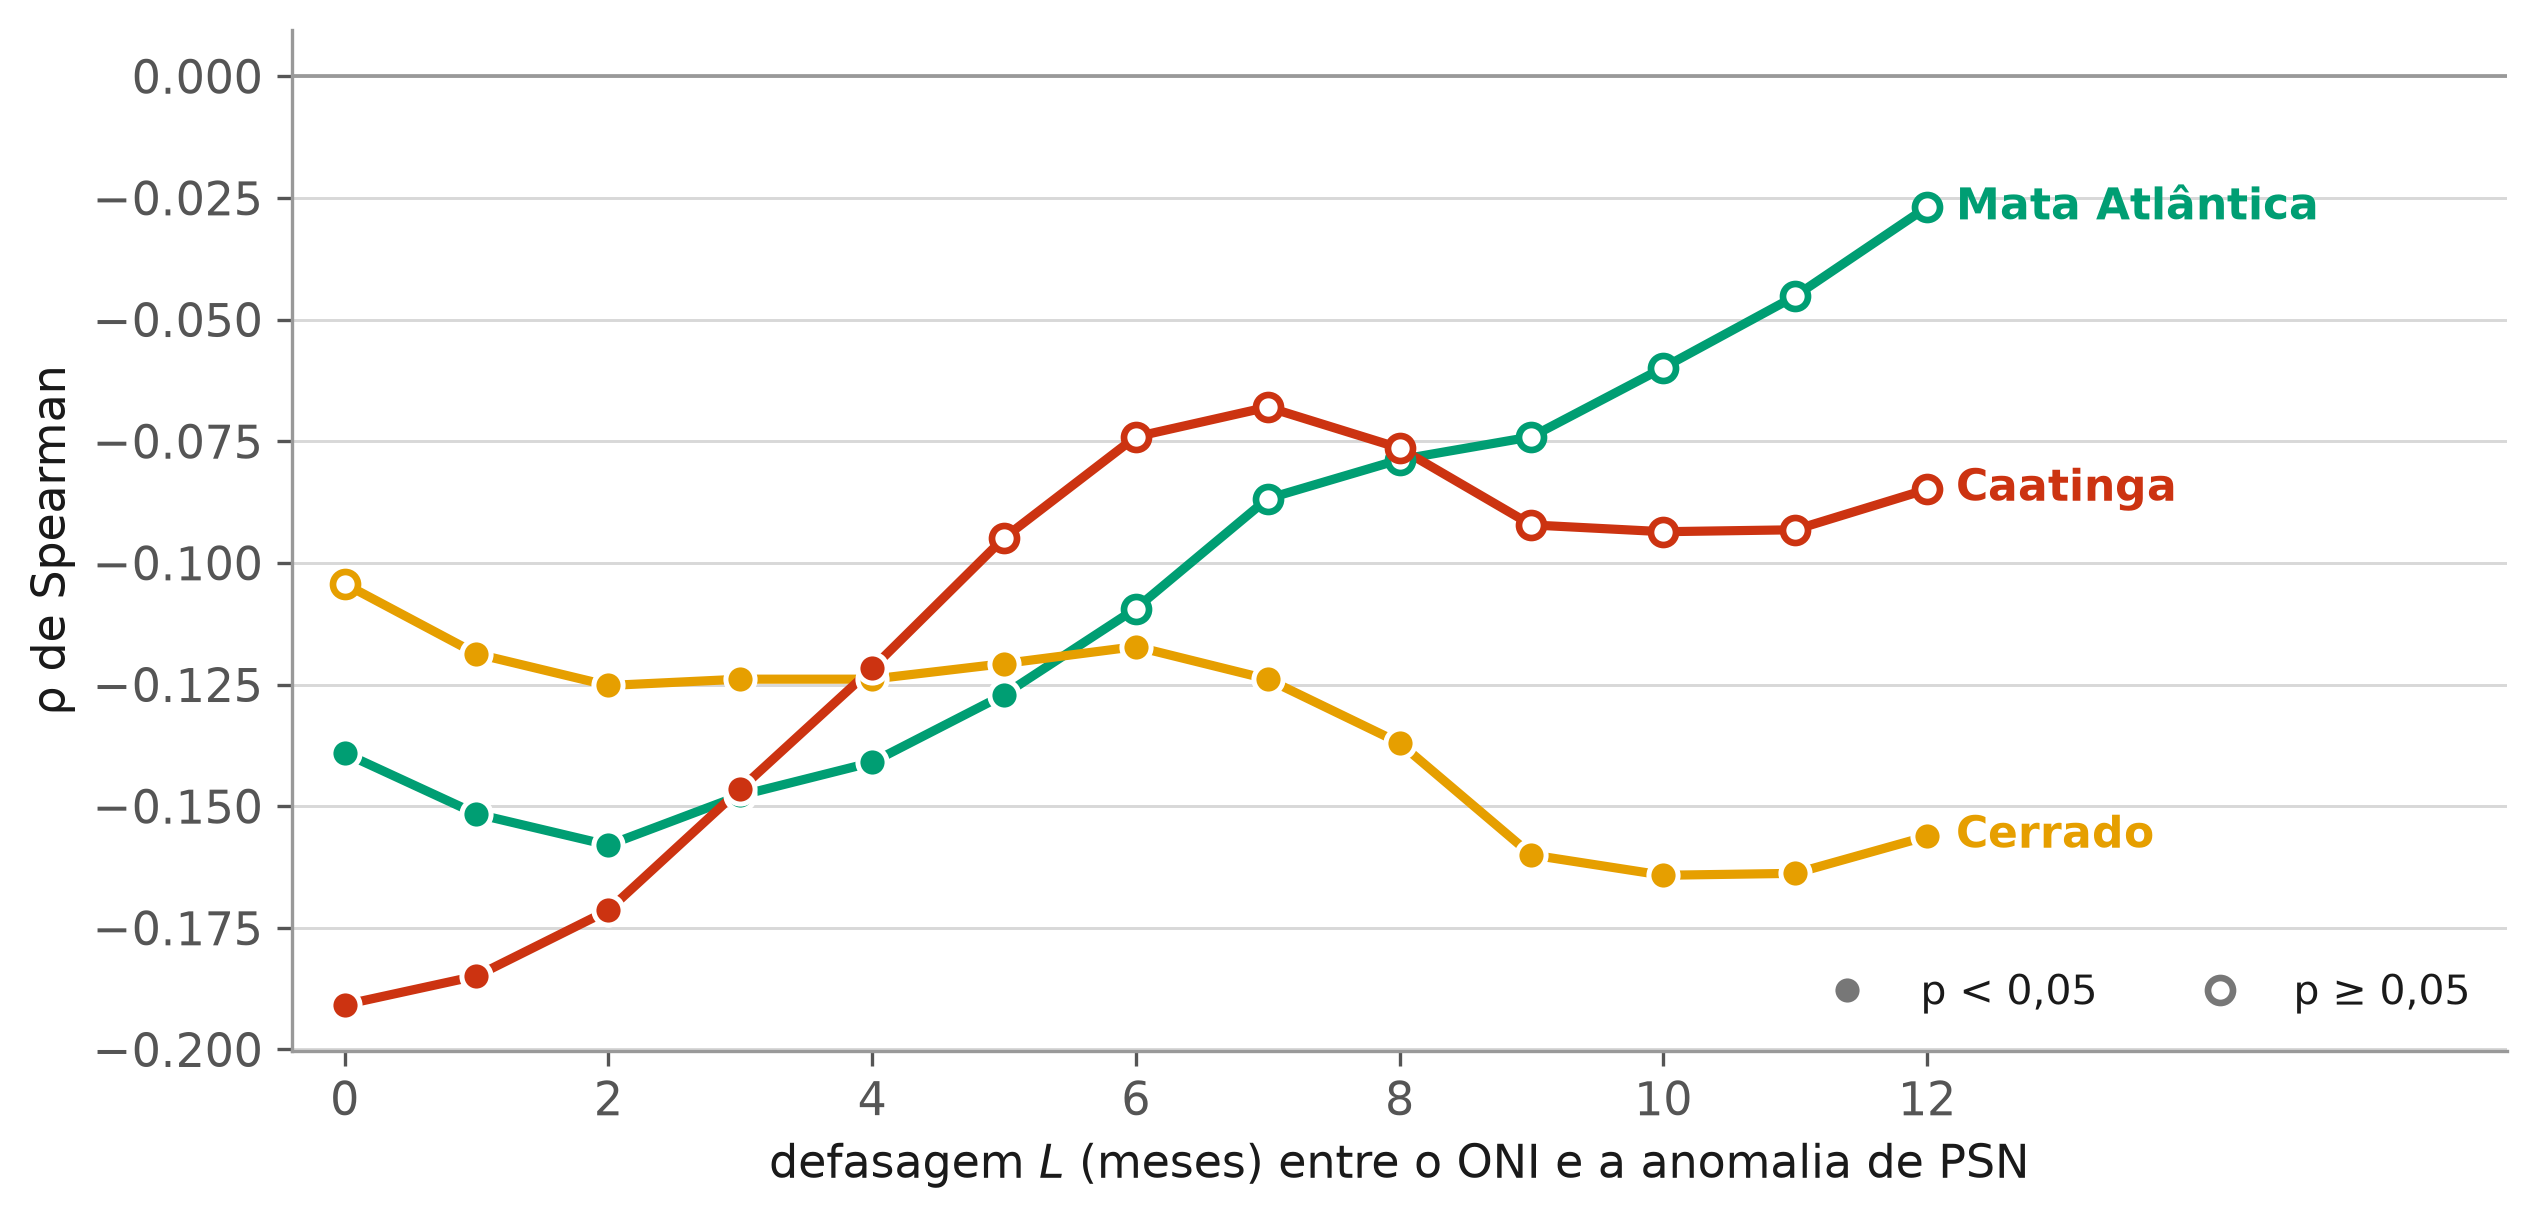
\includegraphics[width=\linewidth]{figs/fig3_defasagem.png}
\caption{Correlação de Spearman entre o ONI do mês $t$ e a anomalia de PSN do mês $t+L$. Os símbolos preenchidos indicam $p < 0{,}05$ sob a premissa de meses independentes.}
\label{fig:defasagem}
\end{figure}

\subsection{Mediação pelo modelo climático}

Impondo ao modelo de regressão polinomial as anomalias médias observadas em cada fase, a resposta predita da PSN reproduz boa parte da observada nas combinações de maior magnitude (Tabela~\ref{tab:mediacao}). Na Caatinga em La Niña, o modelo prediz $+9{,}8\%$ contra $+10{,}4\%$ observados, isto é, 94\% da resposta; no Cerrado na mesma fase, $+8{,}0\%$ contra $+11{,}7\%$, ou 68\%; e na Mata Atlântica em El Niño, $-3{,}1\%$ contra $-5{,}4\%$, ou 57\%. A decomposição por preditor indica que a contribuição vem sobretudo da evapotranspiração nos biomas sazonais ($+9{,}0$ e $+11{,}6$ pontos em La Niña na Caatinga e no Cerrado) e da temperatura da superfície na Mata Atlântica.

\begin{table}[width=\linewidth,cols=5,pos=h]
\caption{Resposta da PSN predita pelo modelo climático quando lhe são impostas as anomalias médias de cada fase, comparada à observada. A coluna final é a razão entre as duas.}
\label{tab:mediacao}
\begin{tabular*}{\tblwidth}{@{}llrrr@{}}
\toprule
Bioma & Fase & Predito (\%) & Observado (\%) & Razão \\
\midrule
Mata Atlântica & El Niño & $-3{,}11$ & $-5{,}44$  & 0,57 \\
Mata Atlântica & La Niña & $+0{,}74$ & $-0{,}08$  & --- \\
Cerrado        & El Niño & $+4{,}48$ & $+5{,}26$  & 0,85 \\
Cerrado        & La Niña & $+8{,}02$ & $+11{,}75$ & 0,68 \\
Caatinga       & El Niño & $-1{,}17$ & $-3{,}28$  & 0,36 \\
Caatinga       & La Niña & $+9{,}84$ & $+10{,}45$ & 0,94 \\
\bottomrule
\end{tabular*}
\end{table}

\subsection{Variabilidade interanual}

Nenhum dos três biomas apresentou tendência significativa da PSN anual entre 2001 e 2024 (Tabela~\ref{tab:interanual}). O declive de Sen foi negativo na Mata Atlântica ($-4{,}3$~gC~m$^{-2}$~ano$^{-1}$, equivalente a $-6{,}2\%$ no período) e positivo no Cerrado ($+11{,}3\%$) e na Caatinga ($+0{,}7\%$), mas os intervalos de confiança cruzam zero em todos os casos e o teste de Mann-Kendall não rejeita a hipótese de ausência de tendência ($p = 0{,}070$, 0,333 e 0,941).

Como verificação de consistência, a soma anual de PSN foi comparada ao NPP anual do produto MOD17A3HGF para as mesmas máscaras de bioma, com correlação de Pearson entre 0,993 e 0,999 nos três casos. A variabilidade interanual é muito desigual entre os biomas: o coeficiente de variação da PSN anual é de 4,6\% na Mata Atlântica, contra 15,0\% no Cerrado e 13,3\% na Caatinga. Os anos extremos não coincidem com as fases do ENSO de forma sistemática. O pior ano da Mata Atlântica, 2016 (1.448~gC~m$^{-2}$~ano$^{-1}$), sucede o El Niño de 2014--2016, mas o melhor ano do Cerrado, 2009 (1.407~gC~m$^{-2}$~ano$^{-1}$), é também um ano de El Niño; e o melhor da Caatinga, 2020 (1.276~gC~m$^{-2}$~ano$^{-1}$), é um ano neutro.

\begin{table}[width=\linewidth,cols=6,pos=h]
\caption{Variabilidade interanual da PSN entre 2001 e 2024. O declive de Sen é expresso em porcentagem do período e testado por Mann-Kendall.}
\label{tab:interanual}
\begin{tabular*}{\tblwidth}{@{}lrrrrr@{}}
\toprule
Bioma & Média & CV & Sen & $p$ & Extremos \\
 & (gC~m$^{-2}$~ano$^{-1}$) & (\%) & (\%) & & (mín/máx) \\
\midrule
Mata Atlântica & 1.604 & 4,6  & $-6{,}2$  & 0,070 & 2016/2014 \\
Cerrado        & 1.157 & 15,0 & $+11{,}3$ & 0,333 & 2002/2009 \\
Caatinga       & 1.044 & 13,3 & $+0{,}7$  & 0,941 & 2012/2020 \\
\bottomrule
\end{tabular*}
\end{table}

\section{Discussão}

O resultado central deste trabalho é a distância entre as duas leituras do mesmo conjunto de dados. Sob o procedimento de uso corrente, 10 dos 30 testes indicam efeito do ENSO, e o padrão que emerge é atraente: a Mata Atlântica responderia à fase quente, o Cerrado e a Caatinga à fase fria, com a resposta propagando-se pela evapotranspiração e pela disponibilidade hídrica. Sob o procedimento que respeita a estrutura temporal dos dados, restam três efeitos, dois deles marginais, e o padrão perde a nitidez. A diferença não vem de dados diferentes, de outra definição de anomalia ou de outra estatística --- $\Delta$ é idêntico nas duas colunas da Tabela~\ref{tab:unidade} ---, mas apenas de reconhecer que os 76 meses de El Niño são 8 episódios.

O alargamento mediano de 1,67 vez nos intervalos é compatível com o esperado. Em blocos de duração média próxima a 9 meses, o tamanho amostral efetivo é uma fração do nominal, e o erro-padrão cresce aproximadamente com a raiz dessa razão. Não se trata, portanto, de um efeito peculiar a esta série: ele deve aparecer sempre que compósitos de fase forem montados sobre observações mensais de episódios plurianuais, o que é a prática usual em estudos de ENSO com dados de sensoriamento remoto. A implicação prática é direta: em séries de 20 a 25 anos, o número de episódios disponíveis é da ordem de uma dezena por fase, e afirmações sobre diferenças de poucos pontos percentuais entre fases dificilmente se sustentam.

Entre os efeitos que resistem, o mais sólido não é de produtividade, mas de temperatura: a superfície da Mata Atlântica ficou 3,1 pontos percentuais acima da anomalia dos meses neutros durante os episódios de El Niño, com intervalo confortavelmente afastado de zero. Isso é coerente com o fato de a teleconexão do ENSO com o Leste do Nordeste brasileiro ser mais consistente na temperatura do que na precipitação \citep{ropelewski1987, kayano2007}. A redução de 5,4\% da PSN no mesmo bioma e fase acompanha esse aquecimento e é parcialmente reproduzida pelo modelo climático, sobretudo pela via térmica --- um resultado compatível com a sensibilidade da fotossíntese à demanda evaporativa em florestas tropicais úmidas \citep{lawson2019, vourlitis2022}.

A ausência de sinal robusto na precipitação merece atenção. A Bahia situa-se em uma zona de transição entre o semiárido setentrional do Nordeste, onde a teleconexão do ENSO com as chuvas é bem documentada, e o Sudeste, onde ela é fraca e de sinal variável \citep{grimm2003, grimm2009}. As médias brutas de precipitação são de fato maiores em La Niña nos três biomas (Tabela~\ref{tab:convencional}), mas a dispersão entre episódios é grande o suficiente para que a diferença não se distinga de zero nem mesmo sob o esquema convencional. A resposta da produtividade que permanece na Caatinga em La Niña ($+10{,}4$~p.p.), portanto, não se deixa atribuir com segurança a um sinal pluviométrico identificado nesta série, ainda que chuvas acima do normal no Brasil Central durante a La Niña sejam bem documentadas em escala regional \citep{cai2020}.

O contraste com a literatura que reporta efeitos fortes e generalizados do ENSO sobre a produtividade \citep{zhao2010, nemani2003} pede cautela na interpretação. Parte dessa literatura opera em escala continental ou global, onde o número efetivo de graus de liberdade é maior porque há replicação espacial além da temporal; parte trabalha com regiões de teleconexão mais forte que a Bahia; e parte adota o mês como unidade, como aqui se fez na primeira análise. Este trabalho não contradiz esses achados: mostra que, para três biomas de um único estado e 24 anos de registro, a evidência disponível é bem mais fraca do que o procedimento convencional sugere.

Algumas limitações devem ser explicitadas. A primeira é que o bootstrap em blocos com 8 ou 9 blocos é ele próprio impreciso: intervalos percentílicos construídos sobre tão poucas unidades têm cobertura apenas aproximada, e os valores de $p$ marginais reportados (0,044 e 0,048) devem ser lidos como indicativos, não como evidência forte. Essa imprecisão, contudo, é a informação honesta sobre o que 24 anos de dados permitem afirmar, e não um defeito do método. A segunda é que a classificação em três fases descarta informação: a intensidade dos episódios, que varia de um ONI de pico de 0,71 a 2,59 na série, não é usada. A terceira é que a análise é correlacional e não separa o efeito do ENSO de outros modos de variabilidade que possam coincidir com ele no período, como a Oscilação Decadal do Pacífico \citep{kayano2007}. A quarta é que a PSN e a evapotranspiração provêm de algoritmos MODIS que compartilham entradas, de modo que a mediação da Tabela~\ref{tab:mediacao} não constitui evidência independente. A quinta é que a temperatura da superfície não passou por filtro de qualidade pela banda QC\_Day, e a sensibilidade da série a esse filtro não foi avaliada.

Duas recomendações decorrem do exposto. A primeira, metodológica: compósitos de fase do ENSO construídos sobre séries mensais devem reportar, além do teste convencional, alguma forma de inferência que respeite a estrutura temporal --- bootstrap em blocos, testes de permutação sobre rótulos de episódio ou correção do tamanho amostral efetivo \citep{kunsch1989, politis1994}. O custo computacional é baixo e a diferença nas conclusões, como se viu, pode ser qualitativa. A segunda, regional: aumentar o número de episódios disponíveis exige estender a série para trás do início do registro MODIS, o que passa por produtos de sensores anteriores ou por reconstruções, ou aumentar a replicação espacial, analisando sub-regiões dentro de cada bioma em vez de uma única média por bioma.

\section{Conclusões}

A fotossíntese líquida dos três biomas da Bahia apresenta, sob o procedimento convencional de compósitos por fase, um padrão assimétrico de resposta ao ENSO, com a Mata Atlântica associada à fase quente e o Cerrado e a Caatinga à fase fria. Quando a unidade amostral passa do mês para o episódio, 7 dos 10 efeitos significativos deixam de ser distinguíveis de zero e os intervalos de confiança alargam-se 1,67 vez em mediana. Permanecem o aquecimento da superfície da Mata Atlântica em El Niño, a redução da PSN nesse bioma e fase e o aumento da PSN da Caatinga em La Niña, os dois últimos marginais. Nenhum bioma apresenta tendência interanual significativa no período. Os resultados indicam que o tratamento dos meses como observações independentes superestima a significância de compósitos do ENSO em séries de sensoriamento remoto e que, com 24 anos de registro e menos de dez episódios por fase, a evidência sobre o efeito do ENSO na produtividade desses biomas é fraca e deve ser apresentada como tal.

\section*{Disponibilidade de dados}
A base mensal (297 períodos por bioma, 2001--2025), o código em Python de todas as análises aqui reportadas e os resultados da rodada completa estão disponíveis em \url{https://github.com/heroslore/MRMP-N-PSN-Bahia} e arquivados de forma permanente no Zenodo sob o DOI \url{https://doi.org/10.5281/zenodo.22883915}, que resolve sempre para a versão mais recente do arquivo. A base é também fornecida como material suplementar (arquivo CSV).

\section*{Declaração de conflito de interesses}
Os autores declaram não haver conflitos de interesse financeiros ou pessoais que pudessem ter influenciado o trabalho relatado neste artigo.

\section*{Agradecimentos}
O presente trabalho foi realizado com apoio da Coordenação de Aperfeiçoamento de Pessoal de Nível Superior -- Brasil (CAPES) -- Código de Financiamento 001, por meio de bolsa de mestrado concedida ao primeiro autor. Os autores agradecem ao Programa de Pós-graduação em Ciências e Tecnologias Ambientais (UFSB/IFBA). O primeiro autor agradece ao Prof. Dr. Fabrício Berton Zanchi, pela orientação, e à Profa. Dra. Nayanne Silva Benfica, pela coorientação.

\section*{CRediT authorship contribution statement}
\textbf{Ygor Augusto dos Santos Oliveira:} Conceituação, Metodologia, Software, Análise formal, Curadoria de dados, Redação -- rascunho original. \textbf{Nayanne Silva Benfica:} Conceituação, Metodologia, Curadoria de dados, Redação -- revisão e edição, Supervisão. \textbf{Fabrício Berton Zanchi:} Conceituação, Metodologia, Redação -- revisão e edição, Supervisão.

\bibliographystyle{cas-model2-names}
\bibliography{refs2}

\end{document}
